% =============================================================================
% SAGAM: A Multi-Modal Interpretable Survival-Aware Generalised Additive
%        Meta-Learner for Lung Adenocarcinoma Prognosis
% Target: IEEE BIBM 2026 / IEEE J. Biomedical and Health Informatics
% Rewritten edition (v3) — figures embedded, numbers reconciled to results_v2/
% =============================================================================
\documentclass[journal]{IEEEtran}

\usepackage{cite}
\usepackage{amsmath,amssymb,amsfonts}
\usepackage{algorithmic}
\usepackage{graphicx}
\usepackage{textcomp}
\usepackage{xcolor}
\usepackage{booktabs}
\usepackage{multirow}
\usepackage{url}
\usepackage{microtype}
\usepackage{array}
\usepackage{siunitx}
\usepackage{tikz}
\usetikzlibrary{arrows.meta,positioning,fit,backgrounds,shapes.geometric}
\usepackage[hidelinks]{hyperref}

\sisetup{detect-weight=true, detect-family=true}
\graphicspath{{../results_v2/}{results_v2/}{./}}

\DeclareMathOperator*{\argmin}{arg\,min}

\begin{document}

% ── Title ────────────────────────────────────────────────────────────────────
\title{SAGAM: A Multi-Modal Interpretable Survival-Aware\\
Generalised Additive Meta-Learner for\\
Lung Adenocarcinoma Prognosis}

\author{%
\IEEEauthorblockN{Lalit Kharel}\\
\IEEEauthorblockA{\textit{Independent Researcher}\\
% Replace the next two lines with your department / institution / city.
\textit{[Department, Institution]}\\
[City, Country] \quad klalit.kharel@gmail.com}%
}

\maketitle

% ── Abstract ─────────────────────────────────────────────────────────────────
\begin{abstract}
Ensemble survival models routinely outperform classical Cox regression on
lung adenocarcinoma (LUAD) cohorts, but they purchase that accuracy with
opacity: a stacked ensemble reports a single risk score and hides
\emph{which} component learner it trusted and \emph{where} along the risk
spectrum. We present \textbf{SAGAM} (Survival-Aware Generalised Additive
Meta-Learner), a multi-modal stacking framework whose meta-learner is a
B-spline generalised additive model (GAM). For each base learner $k$, SAGAM
fits a smooth log-hazard contribution function $f_k(s_k)$ over that learner's
out-of-fold risk score $s_k$. The shapes of these functions are the model's
explanation: steep segments are \emph{trust zones} where the ensemble relies
on learner $k$, and flat segments mark where it is ignored. This replaces the
single scalar weight of linear stacking with a global, continuous, and
clinically inspectable trust structure.

SAGAM stacks five base learners --- Random Survival Forest (RSF), Gradient
Boosting Survival (GBS), XGBoost-Cox, a batch-normalised DeepSurv network, and
a gene-expression-specific CoxNet (ExprCox) --- over a feature space that
fuses 16 clinical/molecular variables with a 10-gene expression panel. Under
strict 5-fold nested cross-validation on TCGA-LUAD ($n{=}497$, 180 events),
Multi-Modal SAGAM reaches a concordance index of
$\mathbf{0.670 \pm 0.023}$, exceeding a clinical-only configuration
($0.620 \pm 0.045$; $\Delta{=}{+}0.050$) while \emph{halving} fold-to-fold
variance, and an expression-only baseline ($0.655 \pm 0.020$). On the fully
independent GSE31210 cohort ($n{=}226$) the expression model attains
$C{=}0.661$ with log-rank $p{=}8.5{\times}10^{-4}$; we additionally report a
negative result on GSE68465 and trace it to gene dropout and platform shift.
Risk tertiles separate median overall survival by $38.7$ months
(71.5 vs.\ 32.8). All code, figures, and trained artefacts are released.
\end{abstract}

\begin{IEEEkeywords}
Survival analysis, lung adenocarcinoma, ensemble stacking, generalised
additive models, B-splines, interpretability, multi-modal integration,
gene expression, TCGA, concordance index.
\end{IEEEkeywords}

% ── I. INTRODUCTION ──────────────────────────────────────────────────────────
\section{Introduction}
\IEEEPARstart{L}{ung} adenocarcinoma (LUAD) is the most common subtype of
non-small-cell lung cancer, representing roughly 40\% of lung cancer
diagnoses and carrying a five-year survival below 25\% in advanced
stages~\cite{siegel2024cancer}. Even after the arrival of EGFR/ALK targeted
therapy and immune-checkpoint blockade, patients with identical TNM stage
follow strikingly different trajectories --- a direct consequence of molecular
heterogeneity that anatomical staging cannot resolve. Better prognostic
stratification is therefore not an academic exercise but a prerequisite for
allocating adjuvant therapy and surveillance.

Machine-learning survival models address this by integrating heterogeneous
data: pathological stage, tumour mutational burden (TMB), genomic-instability
indices, hypoxia scores, and transcriptomic profiles. Two tensions, however,
have repeatedly limited their clinical translation. \emph{First}, the most
accurate methods --- random forests, gradient boosting, deep networks ---
are opaque; clinicians are asked to trust a number with no account of how it
was formed. \emph{Second}, models tuned on a single cohort (typically TCGA)
often collapse on external data because of microarray-platform differences,
missing probes, and population shift, so reported discrimination overstates
real-world reliability.

SAGAM is designed around both tensions at once. Its central idea is to make
\emph{the act of ensembling itself} interpretable. Where conventional stacking
learns one scalar weight per base learner, SAGAM learns a smooth function
$f_k(s_k)$ mapping each learner's risk score to a log-hazard contribution
(Fig.~\ref{fig:arch}). The derivative $|f_k'(s)|$ is a direct, continuous
read-out of trust: where it is large, the ensemble is leaning on learner $k$;
where $f_k\!\approx\!0$, that learner is effectively switched off. We call the
high-derivative segments \emph{trust zones}.

\noindent\textbf{Contributions.}
\begin{enumerate}
  \item \textbf{Interpretable ensembling via B-spline trust functions.}
  We formulate the meta-learner as a B-spline GAM and show that the resulting
  per-learner smooths constitute a global, visualisable trust structure ---
  an explanation that linear stacking and attention-weighted ensembles cannot
  produce. This is the paper's primary contribution.

  \item \textbf{Multi-modal integration with quantified benefit.}
  Fusing clinical features with a 10-gene panel inside one leakage-controlled
  nested-CV pipeline adds $+0.050$ C-index over clinical features alone and
  \emph{halves} fold variance ($\sigma\!:\!0.045\!\to\!0.023$), evidence that
  expression \emph{stabilises} rather than merely augments the clinical signal.

  \item \textbf{Honest external validation.}
  We evaluate on two independent GEO cohorts and report both the success
  (GSE31210) and the failure (GSE68465), attributing the latter to
  identifiable, measurable causes rather than omitting it.
\end{enumerate}

The remainder of the paper reviews related work
(Sec.~\ref{sec:related}), details the architecture (Sec.~\ref{sec:method}),
specifies the experimental protocol (Sec.~\ref{sec:exp}), reports results
(Sec.~\ref{sec:results}), and discusses limitations and outlook
(Sec.~\ref{sec:discussion}--\ref{sec:conclusion}).

% ── Architecture figure (TikZ — self-contained, no external file) ─────────────
\begin{figure*}[!t]
\centering
\resizebox{\textwidth}{!}{%
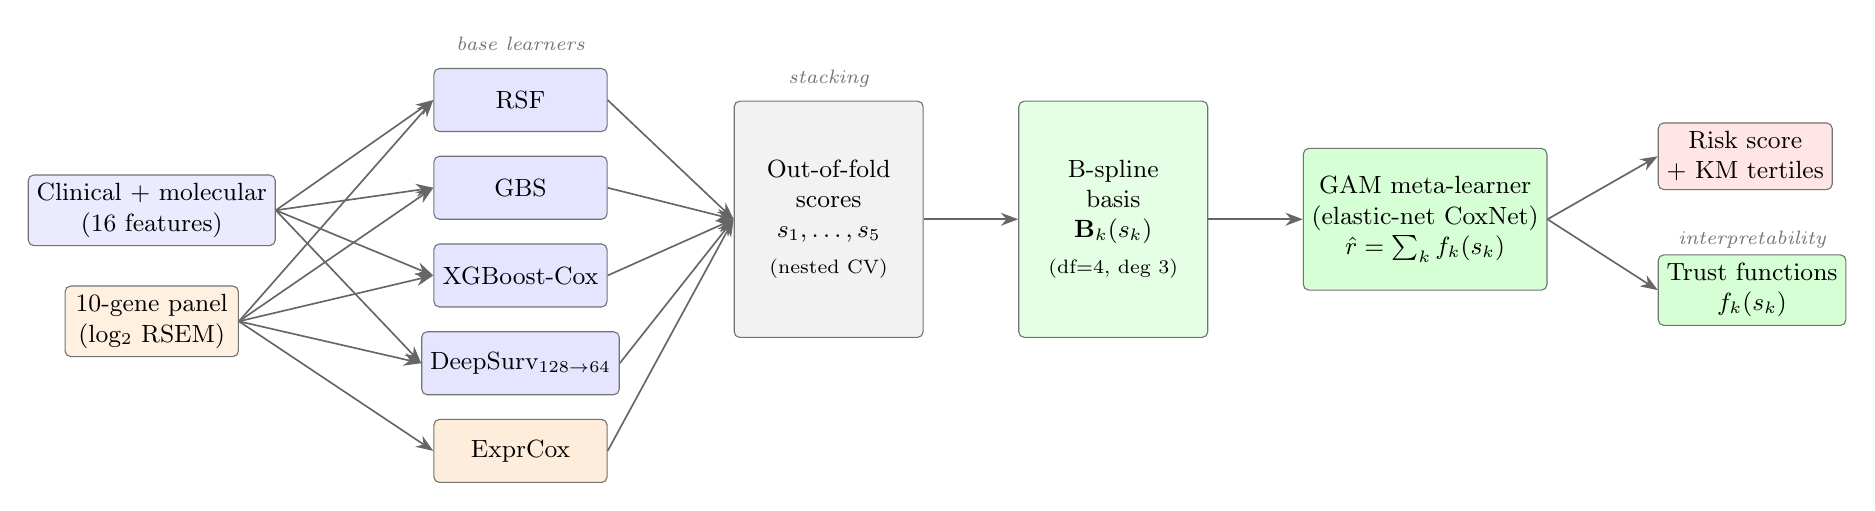
\begin{tikzpicture}[
  font=\small,
  box/.style={rounded corners=2pt, draw=black!55, fill=#1, minimum height=8mm,
              minimum width=22mm, align=center, inner sep=3pt},
  arr/.style={-{Stealth[length=2.2mm]}, draw=black!60, line width=0.6pt},
  lab/.style={font=\scriptsize\itshape, text=black!55}
]
% Data sources
\node[box=blue!8] (clin) {Clinical + molecular\\(16 features)};
\node[box=orange!12, below=5mm of clin] (expr) {10-gene panel\\(log$_2$ RSEM)};

% Base learners
\node[box=blue!10, right=20mm of clin, yshift=14mm] (rsf) {RSF};
\node[box=blue!10, below=3mm of rsf] (gbs) {GBS};
\node[box=blue!10, below=3mm of gbs] (xgb) {XGBoost-Cox};
\node[box=blue!10, below=3mm of xgb] (ds)  {DeepSurv$_{128\to64}$};
\node[box=orange!14, below=3mm of ds] (ec) {ExprCox};

% OOF
\node[box=gray!10, right=16mm of gbs, yshift=-4mm, minimum height=30mm,
      minimum width=24mm] (oof) {Out-of-fold\\scores\\$s_1,\dots,s_5$\\[2pt]\scriptsize(nested CV)};

% Spline expansion
\node[box=green!10, right=12mm of oof, minimum height=30mm, minimum width=24mm]
     (spl) {B-spline\\basis\\$\mathbf{B}_k(s_k)$\\[2pt]\scriptsize(df$=$4, deg 3)};

% GAM meta
\node[box=green!16, right=12mm of spl, minimum height=18mm] (gam)
     {GAM meta-learner\\(elastic-net CoxNet)\\$\hat r=\sum_k f_k(s_k)$};

% Outputs
\node[box=red!10, right=14mm of gam, yshift=8mm] (risk) {Risk score\\+ KM tertiles};
\node[box=green!16, right=14mm of gam, yshift=-9mm] (interp)
     {Trust functions\\$f_k(s_k)$};

% Edges
\foreach \s in {clin,expr} {
  \draw[arr] (\s.east) -- (rsf.west);
  \draw[arr] (\s.east) -- (gbs.west);
  \draw[arr] (\s.east) -- (xgb.west);
  \draw[arr] (\s.east) -- (ds.west);
}
\draw[arr] (expr.east) -- (ec.west);
\foreach \b in {rsf,gbs,xgb,ds,ec} { \draw[arr] (\b.east) -- (oof.west); }
\draw[arr] (oof.east) -- (spl.west);
\draw[arr] (spl.east) -- (gam.west);
\draw[arr] (gam.east) -- (risk.west);
\draw[arr] (gam.east) -- (interp.west);

\node[lab, above=1mm of rsf] {base learners};
\node[lab, above=0.5mm of oof] {stacking};
\node[lab, above=0.5mm of interp, yshift=-1mm] {interpretability};
\end{tikzpicture}}
\caption{SAGAM architecture. Five base learners are trained on the fused
clinical+expression feature space (ExprCox on the 10-gene panel only). Their
leakage-free out-of-fold risk scores are expanded into cubic B-spline bases and
fed to an elastic-net CoxNet GAM meta-learner. The meta-learner emits both a
patient risk score and, as a by-product of its coefficients, the per-learner
trust functions $f_k(s_k)$.}
\label{fig:arch}
\end{figure*}

% ── II. RELATED WORK ─────────────────────────────────────────────────────────
\section{Related Work}
\label{sec:related}

\subsection{Survival Models in Oncology}
The Cox proportional-hazards model~\cite{cox1972regression} assumes a
log-linear covariate--hazard relationship; CoxNet adds LASSO/elastic-net
regularisation for high-dimensional genomic data~\cite{simon2011regularization}.
These models are interpretable but cannot represent the nonlinear
interactions that characterise tumour biology. Random Survival
Forests~\cite{ishwaran2008random}, Gradient Boosting
Survival~\cite{hothorn2006survival}, XGBoost-Cox~\cite{chen2016xgboost}, and
DeepSurv~\cite{katzman2018deepsurv} recover such nonlinearity and improve
discrimination, but each is, on its own, a black box.

\subsection{Ensemble Stacking for Survival}
Stacking (super-learning)~\cite{van2007super} trains a meta-learner on
out-of-fold (OOF) base-learner predictions to combine complementary strengths.
For survival endpoints, linear CoxNet meta-learners have been
used~\cite{polley2010super}, but they assign a single static weight per
learner and so cannot express the fact that a learner may be reliable in one
region of the risk spectrum and uninformative in another. SAGAM's contribution
is precisely to make those weights \emph{functions} of the risk score.

\subsection{Gene-Expression Signatures and Portability}
Prognostic LUAD expression signatures have been proposed across many
platforms~\cite{shedden2008gene,beer2002gene}, yet portability --- the
attenuation of a signature when moved to a different microarray platform ---
remains a core obstacle~\cite{luo2010comparison}. We measure this directly by
evaluating one fixed 10-gene panel on two cohorts profiled on different
Affymetrix platforms (HG-U133A vs.\ HG-U133 Plus 2.0).

\subsection{Interpretability for Survival}
Post-hoc tools such as SHAP~\cite{lundberg2017unified} and partial-dependence
plots~\cite{friedman2001greedy} explain individual predictions of a fixed
model, and additive-hazard models~\cite{aalen1989linear} expose covariate
effects. None of these characterise the \emph{ensemble trust structure} ---
how the combiner's reliance on each component varies with predicted risk.
SAGAM's smooth contribution functions fill that gap in a principled way.

% ── III. METHODOLOGY ─────────────────────────────────────────────────────────
\section{Methodology}
\label{sec:method}

\subsection{Problem Formulation}
Let $\mathcal{D}=\{(\mathbf{x}_i,t_i,\delta_i)\}_{i=1}^N$ be a right-censored
survival dataset with covariates $\mathbf{x}_i\in\mathbb{R}^p$, observed time
$t_i\in\mathbb{R}^{+}$, and event indicator $\delta_i\in\{0,1\}$ (1 = death).
We seek a risk function $\hat r:\mathbb{R}^p\!\to\!\mathbb{R}$ ordering patients
by hazard.

\subsection{Multi-Modal Feature Space}
\label{sec:features}
The covariate vector combines two modalities.
\textbf{Clinical (16 variables):} AJCC pathological stage, T/N/M substages,
age, sex, grade, ethnicity, prior diagnosis, body weight, aneuploidy score,
MSI-MANTIS, MSIsensor, TMB, tumour break load, and Buffa/Winter/Ragnum hypoxia
scores. \textbf{Expression (10 genes):} DKK1, FAM83A, RHOV, IRX5, SFTA3, CD1B,
PKP2, TNS4, LYPD3, TFAP2A --- a panel chosen for established prognostic
relevance in LUAD, spanning the immune microenvironment (CD1B), invasion
(RHOV, LYPD3), and Wnt/EGFR signalling (DKK1, FAM83A). RSEM counts are
$\log_2(x{+}1)$-transformed.

\subsection{Base-Learner Suite}
\label{sec:base}
Five base learners receive the fused feature set, except ExprCox, which uses
the 10 expression features only:
\begin{enumerate}
  \item \textbf{RSF}: 200 trees, $\sqrt{p}$ features/split, min.\ leaf 5.
  \item \textbf{GBS}: 200 stages, learning rate $0.05$, max depth 3.
  \item \textbf{XGBoost-Cox}: \texttt{survival:cox}, $\eta{=}0.05$, depth 3,
        row/column subsample $0.8$, up to 300 rounds with early stopping
        (patience 20) on a held-out set.
  \item \textbf{DeepSurv}: two fully connected blocks
        ($128\!\to\!64$) each with batch normalisation, ReLU and dropout
        ($p{=}0.3$), trained on the Cox partial-likelihood with Adam
        ($\mathrm{lr}{=}10^{-3}$, weight decay $10^{-4}$), $\leq300$ epochs,
        early stopping patience 25.
  \item \textbf{ExprCox}: elastic-net CoxNet ($\ell_1$-ratio $0.9$) on the
        10-gene panel; the penalty $\alpha$ is tuned on a 20\% internal split.
\end{enumerate}

\subsection{Leakage-Free Nested Cross-Validation}
\label{sec:nested_cv}
Valid stacking requires that the OOF scores training the meta-learner never
come from samples a base learner saw. We enforce this with the design in
Fig.~\ref{fig:arch}:
\begin{enumerate}
  \item \emph{Outer loop}: 5-fold StratifiedKFold (stratified on $\delta$,
        seed 42); each fold yields a held-out test set $\mathcal{T}_k$.
  \item \emph{Early-stopping isolation}: a disjoint set $\mathcal{E}$
        ($15\%$ of the training fold, $\geq10$ samples) is carved off
        \emph{before} the inner loop and used only for XGBoost/DeepSurv
        early stopping --- never for OOF generation or meta-training.
  \item \emph{Inner loop}: 3-fold KFold on the remaining training data
        produces the OOF score matrix.
  \item \emph{Meta-training}: the GAM is fit on OOF scores; its penalty is
        tuned on a held-out 20\% of those scores.
  \item \emph{Test}: base learners are refit on the full inner-training data,
        and the frozen GAM scores $\mathcal{T}_k$. Test samples touch no
        fitting or tuning step.
\end{enumerate}
All preprocessing (one-hot encoding with first-level drop, median imputation,
standardisation) is fit on training folds only.

\subsection{B-Spline GAM Meta-Learner}
\label{sec:gam}
Let $s_k\in\mathbb{R}^N$ be the OOF risk-score vector of learner $k$. SAGAM
expands each $s_k$ into $J{=}4$ cubic B-spline basis functions
$\{B_{kj}(s_k)\}_{j=1}^{J}$ (degree 3, no intercept) and concatenates them:
\begin{equation}
  \mathbf{Z}=[\mathbf{B}_1(s_1),\,\mathbf{B}_2(s_2),\,\dots,\,\mathbf{B}_K(s_K)]
  \in\mathbb{R}^{N\times KJ}.
  \label{eq:spline_matrix}
\end{equation}
An elastic-net Cox model ($\ell_1$-ratio $0.9$) is fit on $\mathbf{Z}$:
\begin{equation}
  \hat{\boldsymbol{\beta}}=\argmin_{\boldsymbol{\beta}}
  \Big[-\ell_{\mathrm{Cox}}(\boldsymbol{\beta};\mathbf{Z})
  +\lambda\big(\alpha\|\boldsymbol{\beta}\|_1
  +\tfrac{1-\alpha}{2}\|\boldsymbol{\beta}\|_2^2\big)\Big].
  \label{eq:coxnet}
\end{equation}
The smooth contribution of learner $k$ is
\begin{equation}
  f_k(s)=\sum_{j=1}^{J}\hat\beta_{kj}\,B_{kj}(s),
  \label{eq:smooth}
\end{equation}
and a new patient's risk is $\hat r=\sum_k f_k(\hat s_k)$, with test scores
$\hat s_k$ clipped to the training range to avoid spline extrapolation.

\noindent\textbf{Interpretation.} Large $|f_k'(s)|$ marks a \emph{trust zone}:
the meta-learner treats learner $k$ as informative at score $s$. Flat segments
($f_k\!\approx\!0$) mean learner $k$ is deferred. Because each $f_k$ is a
single continuous curve over the whole risk range, it offers a global account
of ensemble behaviour --- distinct from, and complementary to, per-patient
attributions such as SHAP.

% ── IV. EXPERIMENTAL SETUP ───────────────────────────────────────────────────
\section{Experimental Setup}
\label{sec:exp}

\subsection{Datasets}
\textbf{TCGA-LUAD (training).} Clinical and RNA-seq data from cBioPortal
(PanCanAtlas 2018). After merging clinical records with the 10-gene panel and
keeping valid endpoints ($t_i{>}0$), the multi-modal cohort has $N{=}497$
patients and 180 events (event rate 36.2\%).\footnote{The clinical cohort
(valid endpoints, no expression requirement) comprises 501 patients (181
events); the multi-modal cohort is obtained by an inner join with RNA-seq,
which drops the 4 patients lacking panel-gene expression (one an event),
giving $N{=}497$ (180 events). All multi-modal, KM, and interpretability
results use the 497-patient cohort; clinical-only baselines use the 501.}

\textbf{GSE31210 (external 1).} 226 patients, surgically resected early-stage
LUAD (Okayama et al., 2012), Affymetrix HG-U133A; all 10 panel genes present;
35 events (15.5\%).

\textbf{GSE68465 (external 2).} 432 patients, Affymetrix HG-U133 Plus 2.0; only
7 of 10 panel genes present (FAM83A, SFTA3, IRX5 absent); 226 events (52.3\%).
Dataset characteristics are summarised in Table~\ref{tab:data}.

\begin{table}[!t]
\centering
\caption{Dataset characteristics.}
\label{tab:data}
\begin{tabular}{lcccl}
\toprule
\textbf{Cohort} & \textbf{$n$} & \textbf{Events} & \textbf{Rate} & \textbf{Platform}\\
\midrule
TCGA-LUAD     & 497 & 180 & 36.2\% & cBio + RNA-seq \\
GSE31210      & 226 & 35  & 15.5\% & Affy HG-U133A \\
GSE68465      & 432 & 226 & 52.3\% & Affy HG-U133 Plus 2.0 \\
\bottomrule
\end{tabular}
\end{table}

\subsection{Evaluation Metrics}
We report Harrell's concordance index (C-index)~\cite{harrell1982evaluating}
as the primary discrimination metric (0.5 random, values 0.65--0.70 clinically
useful); the Integrated Brier Score (IBS)~\cite{graf1999assessment} for
calibration (0.25 = uninformative); IPCW time-dependent
AUC~\cite{uno2007evaluating} at 1/3/5 years; the log-rank test for tertile
separation; and multivariate-Cox hazard ratios (HR) on tertile assignment.
Confidence intervals on external cohorts use 1000-sample bootstrap.

\subsection{Comparators}
Stage-only Cox; Clinical CoxNet; Clinical+Genomic CoxNet; each individual base
learner; linear stacking (CoxNet on raw base scores, no spline expansion);
Clinical-only SAGAM; and Expression-only CoxNet.

% ── V. RESULTS ───────────────────────────────────────────────────────────────
\section{Results}
\label{sec:results}

\subsection{Three-Way Nested-CV Comparison}
Table~\ref{tab:3way} reports the primary discrimination results.
Multi-Modal SAGAM achieves $0.670\pm0.023$, exceeding Clinical-only SAGAM
($0.620\pm0.045$) by $+0.050$ and Expression-only CoxNet ($0.655\pm0.020$) by
$+0.015$. Crucially, the fold-level standard deviation drops from $0.045$
(clinical) to $0.023$ (multi-modal) --- a 50\% variance reduction. The
per-fold values (Table~\ref{tab:folds}) make this concrete: the clinical model
swings from $0.586$ to $0.708$, whereas the multi-modal model stays within
$0.635$--$0.700$. Expression features thus \emph{stabilise} the estimator in
folds where clinical staging is weakly discriminative, rather than simply
adding signal on average.

\begin{table}[!t]
\centering
\caption{Three-way nested-CV comparison --- TCGA-LUAD ($n{=}497$, 180 events).}
\label{tab:3way}
\begin{tabular}{lccc}
\toprule
\textbf{Model} & \textbf{Mean C} & \textbf{SD} & \textbf{$\Delta$ vs Clin.}\\
\midrule
Expression-only            & 0.6549 & 0.0201 & $+0.035$ \\
Clinical-only SAGAM        & 0.6197 & 0.0447 & --- \\
\textbf{Multi-Modal SAGAM} & \textbf{0.6700} & \textbf{0.0225} & $\mathbf{+0.050}$ \\
\midrule
Stage-only Cox             & 0.6542 & 0.0511 & $+0.034$ \\
Clinical CoxNet            & 0.6455 & 0.0279 & $+0.026$ \\
Clinical+Genomic CoxNet    & 0.6412 & 0.0322 & $+0.022$ \\
Linear Stacking            & 0.6274 & 0.0550 & $+0.008$ \\
\midrule
RSF / GBS / XGB / DeepSurv & \multicolumn{3}{c}{$0.619$ / $0.605$ / $0.602$ / $0.636$}\\
\bottomrule
\end{tabular}
\end{table}

\begin{table}[!t]
\centering
\caption{Per-fold C-indices (5-fold StratifiedKFold).}
\label{tab:folds}
\begin{tabular}{lcccccc}
\toprule
\textbf{Model} & \textbf{F1} & \textbf{F2} & \textbf{F3} & \textbf{F4} & \textbf{F5} & \textbf{Mean}\\
\midrule
Expression-only     & 0.666 & 0.651 & 0.655 & 0.621 & 0.682 & 0.655 \\
Clinical-only SAGAM & 0.708 & 0.586 & 0.593 & 0.607 & 0.605 & 0.620 \\
Multi-Modal SAGAM   & 0.700 & 0.635 & 0.678 & 0.656 & 0.682 & \textbf{0.670} \\
\bottomrule
\end{tabular}
\end{table}

\subsection{Comparison with Cox and Stacking Baselines}
Multi-Modal SAGAM ($0.670$) exceeds Stage-only Cox ($0.654$, the principal
clinical benchmark) by $+0.016$, Clinical CoxNet ($0.646$) by $+0.025$, and
linear stacking ($0.627$) by $+0.043$. The gap over linear stacking is the key
methodological signal: replacing scalar weights with spline trust functions,
holding the base learners fixed, yields the largest single improvement
(Fig.~\ref{fig:bar}).

\begin{figure}[!t]
\centering
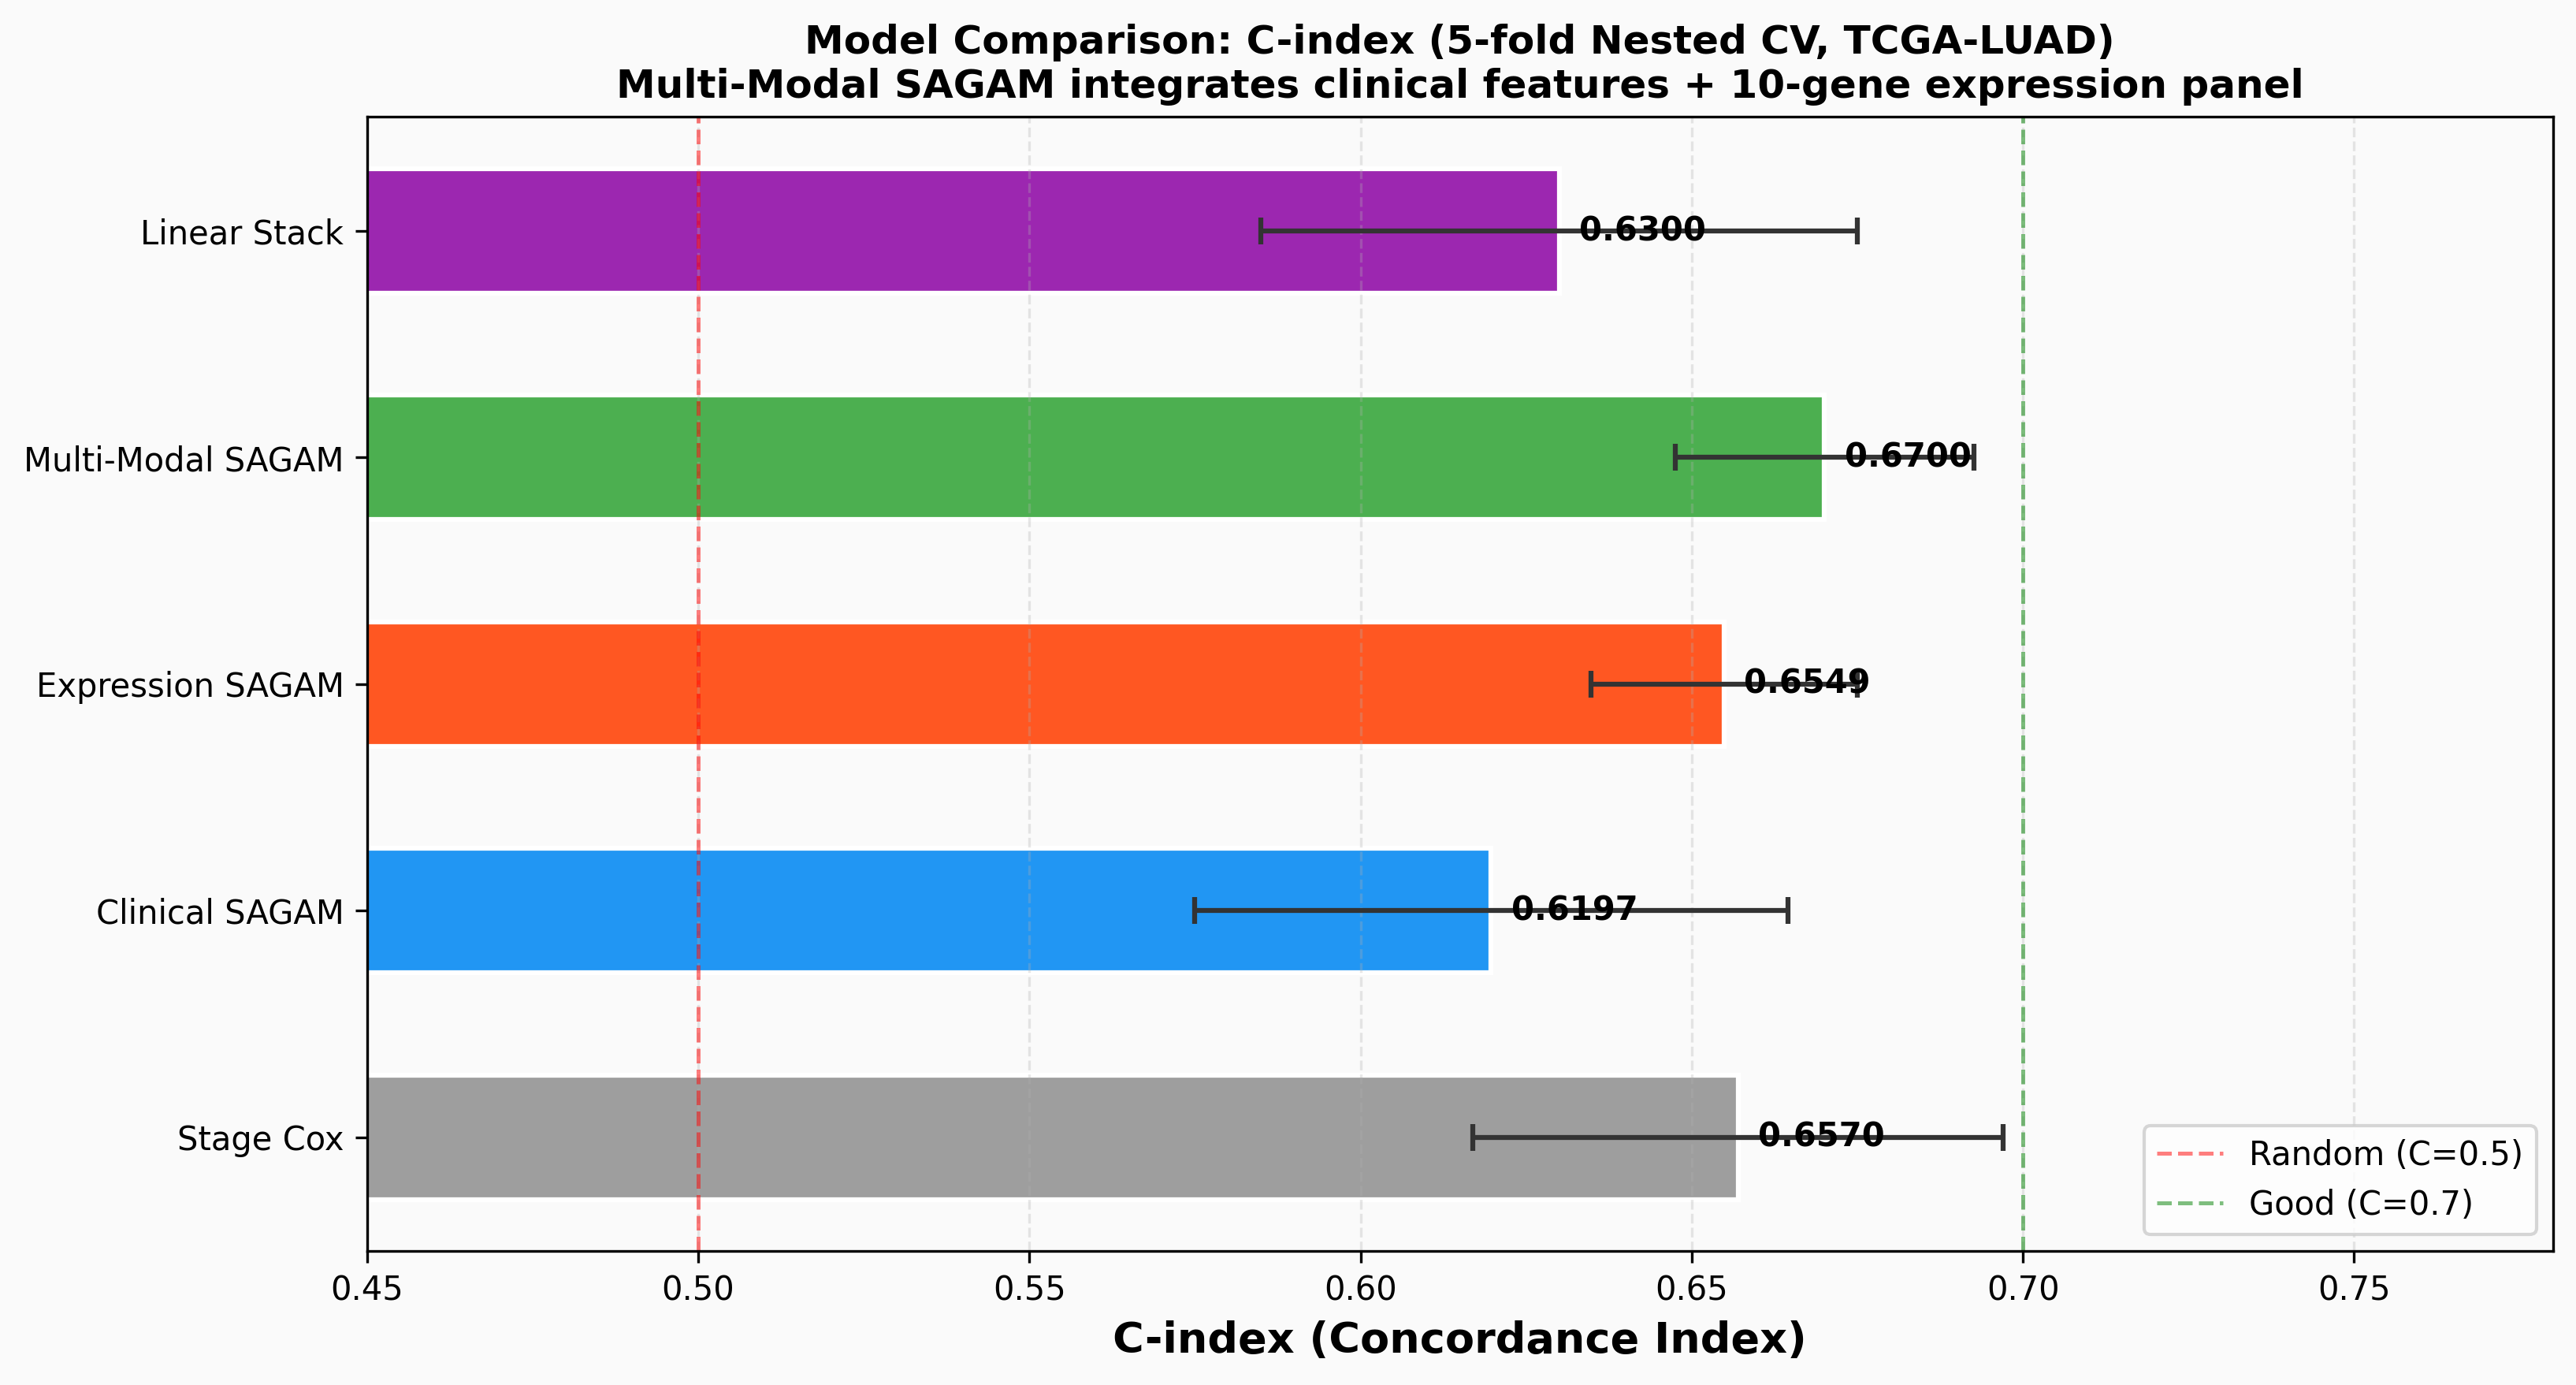
\includegraphics[width=\columnwidth]{model_comparison_bar.png}
\caption{Mean nested-CV C-index across models. SAGAM's gain over linear
stacking isolates the contribution of the B-spline trust functions, since both
share identical base learners and OOF scores.}
\label{fig:bar}
\end{figure}

\subsection{Time-Dependent AUC and Calibration}
Table~\ref{tab:tdauc} gives IPCW time-dependent AUC. SAGAM is competitive at
the 5-year horizon ($0.659$) but lower at 1 year ($0.635$) than Stage Cox
($0.700$) and linear stacking ($0.672$). This is consistent with a rank-based
meta-objective (Cox partial likelihood) that optimises long-horizon ordering
rather than calibrated short-term probabilities; the Breslow baseline applied
to OOF scores is the likely source of the early-horizon gap. Component
calibration is adequate --- RSF IBS $=0.188$ and GBS IBS $=0.194$, both well
below the uninformative $0.25$ --- and Fig.~\ref{fig:calib} shows the
multi-modal risk ranks track observed Kaplan--Meier survival across bins.

\begin{table}[!t]
\centering
\caption{IPCW time-dependent AUC at 1-, 3-, 5-year horizons.}
\label{tab:tdauc}
\begin{tabular}{lccc}
\toprule
\textbf{Model} & \textbf{1-Year} & \textbf{3-Year} & \textbf{5-Year}\\
\midrule
Stage Cox       & 0.700 & 0.663 & 0.619 \\
Clinical Cox    & 0.664 & 0.675 & 0.653 \\
RSF             & 0.667 & 0.695 & 0.705 \\
GBS             & 0.640 & 0.683 & 0.636 \\
XGBoost-Cox     & 0.515 & 0.678 & 0.628 \\
DeepSurv        & 0.648 & 0.678 & 0.710 \\
Linear Stacking & 0.672 & 0.688 & 0.694 \\
SAGAM           & 0.635 & 0.632 & 0.659 \\
\bottomrule
\end{tabular}
\end{table}

\begin{figure}[!t]
\centering
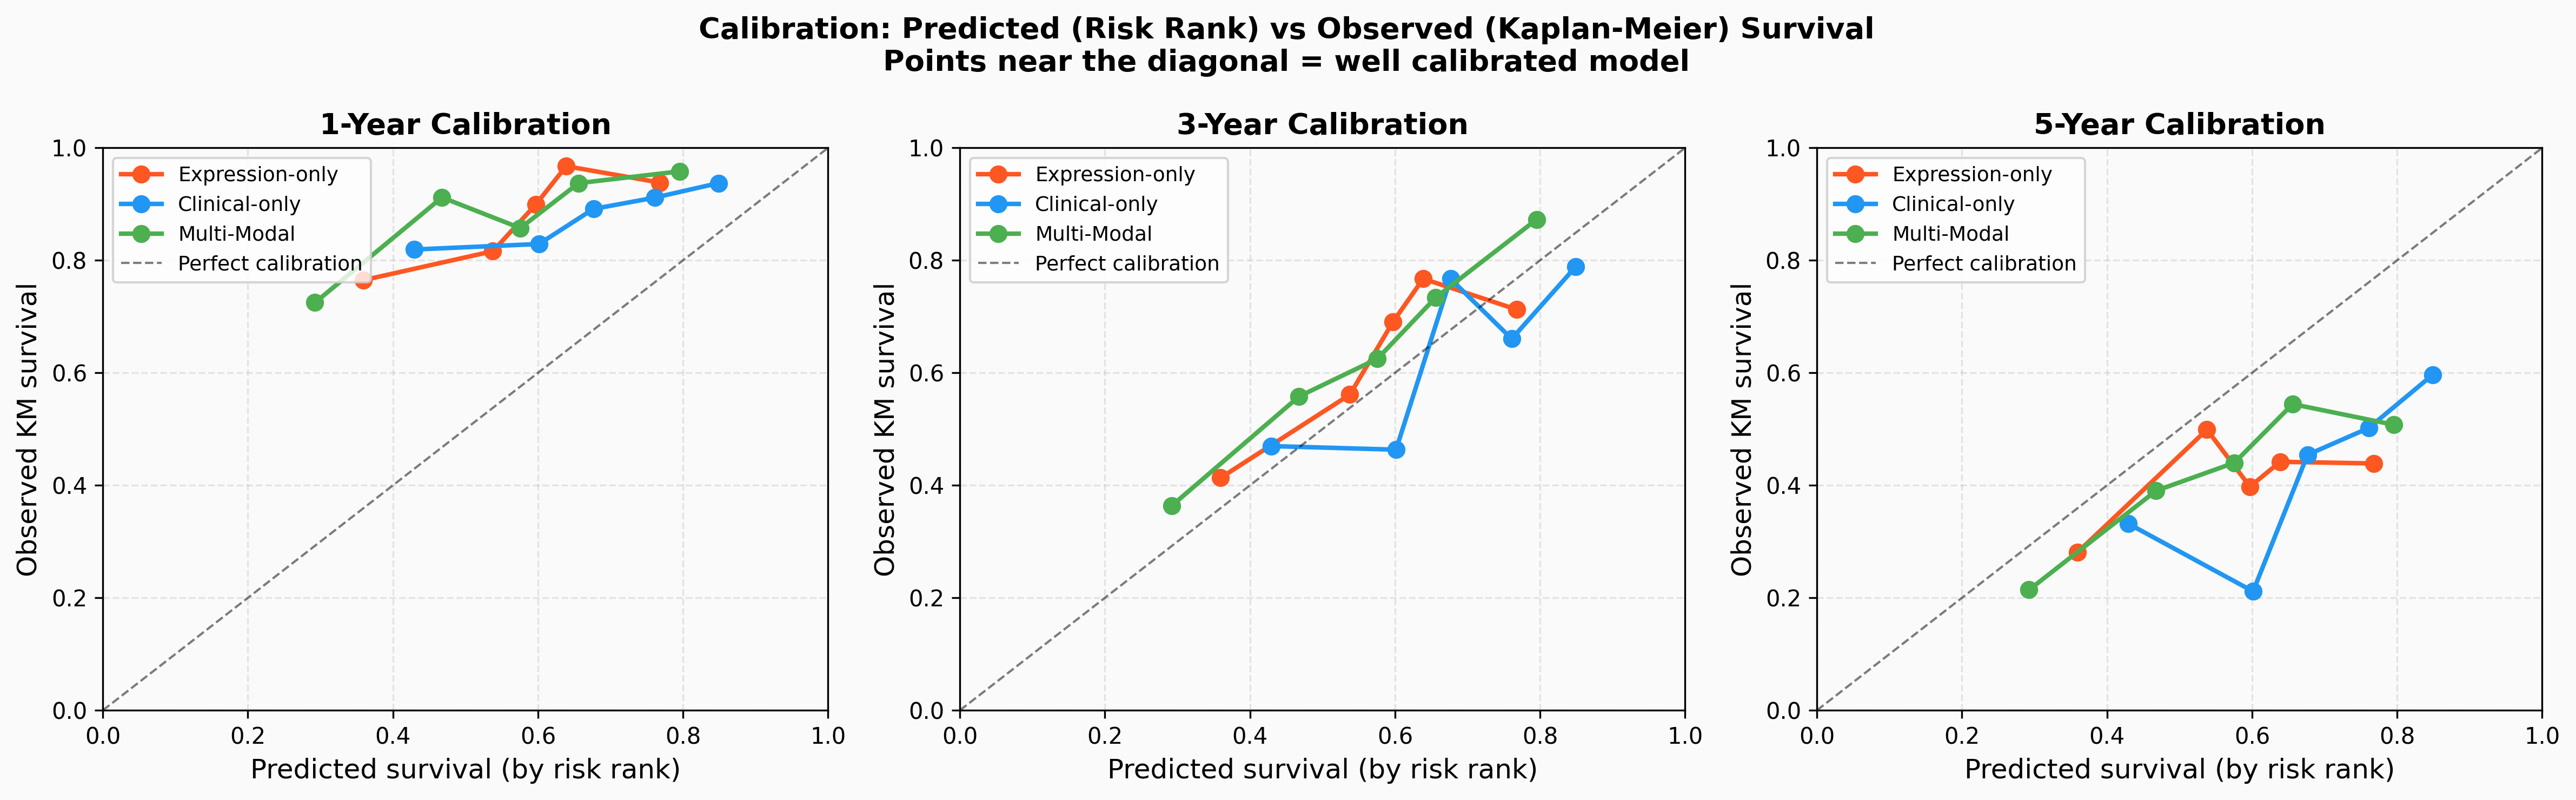
\includegraphics[width=\columnwidth]{calibration_curves.png}
\caption{Calibration at 1/3/5 years: observed Kaplan--Meier survival per
risk-rank bin against predicted ordering for the three configurations. Points
near the diagonal indicate the ordering is consistent with observed survival.}
\label{fig:calib}
\end{figure}

\subsection{Kaplan--Meier Risk Stratification}
Pooled OOF scores from Multi-Modal SAGAM split TCGA-LUAD into tertiles with
clearly separated survival (Fig.~\ref{fig:km}, Table~\ref{tab:km}): median
overall survival of 71.5, 49.3 and 32.8 months for Low/Medium/High risk ---
a 38.7-month spread between the extremes. The log-rank test (Low vs.\ High)
gives $p<0.001$, and multivariate Cox yields HR $=0.375$
(95\% CI 0.257--0.547) for Low vs.\ High.

\begin{figure}[!t]
\centering
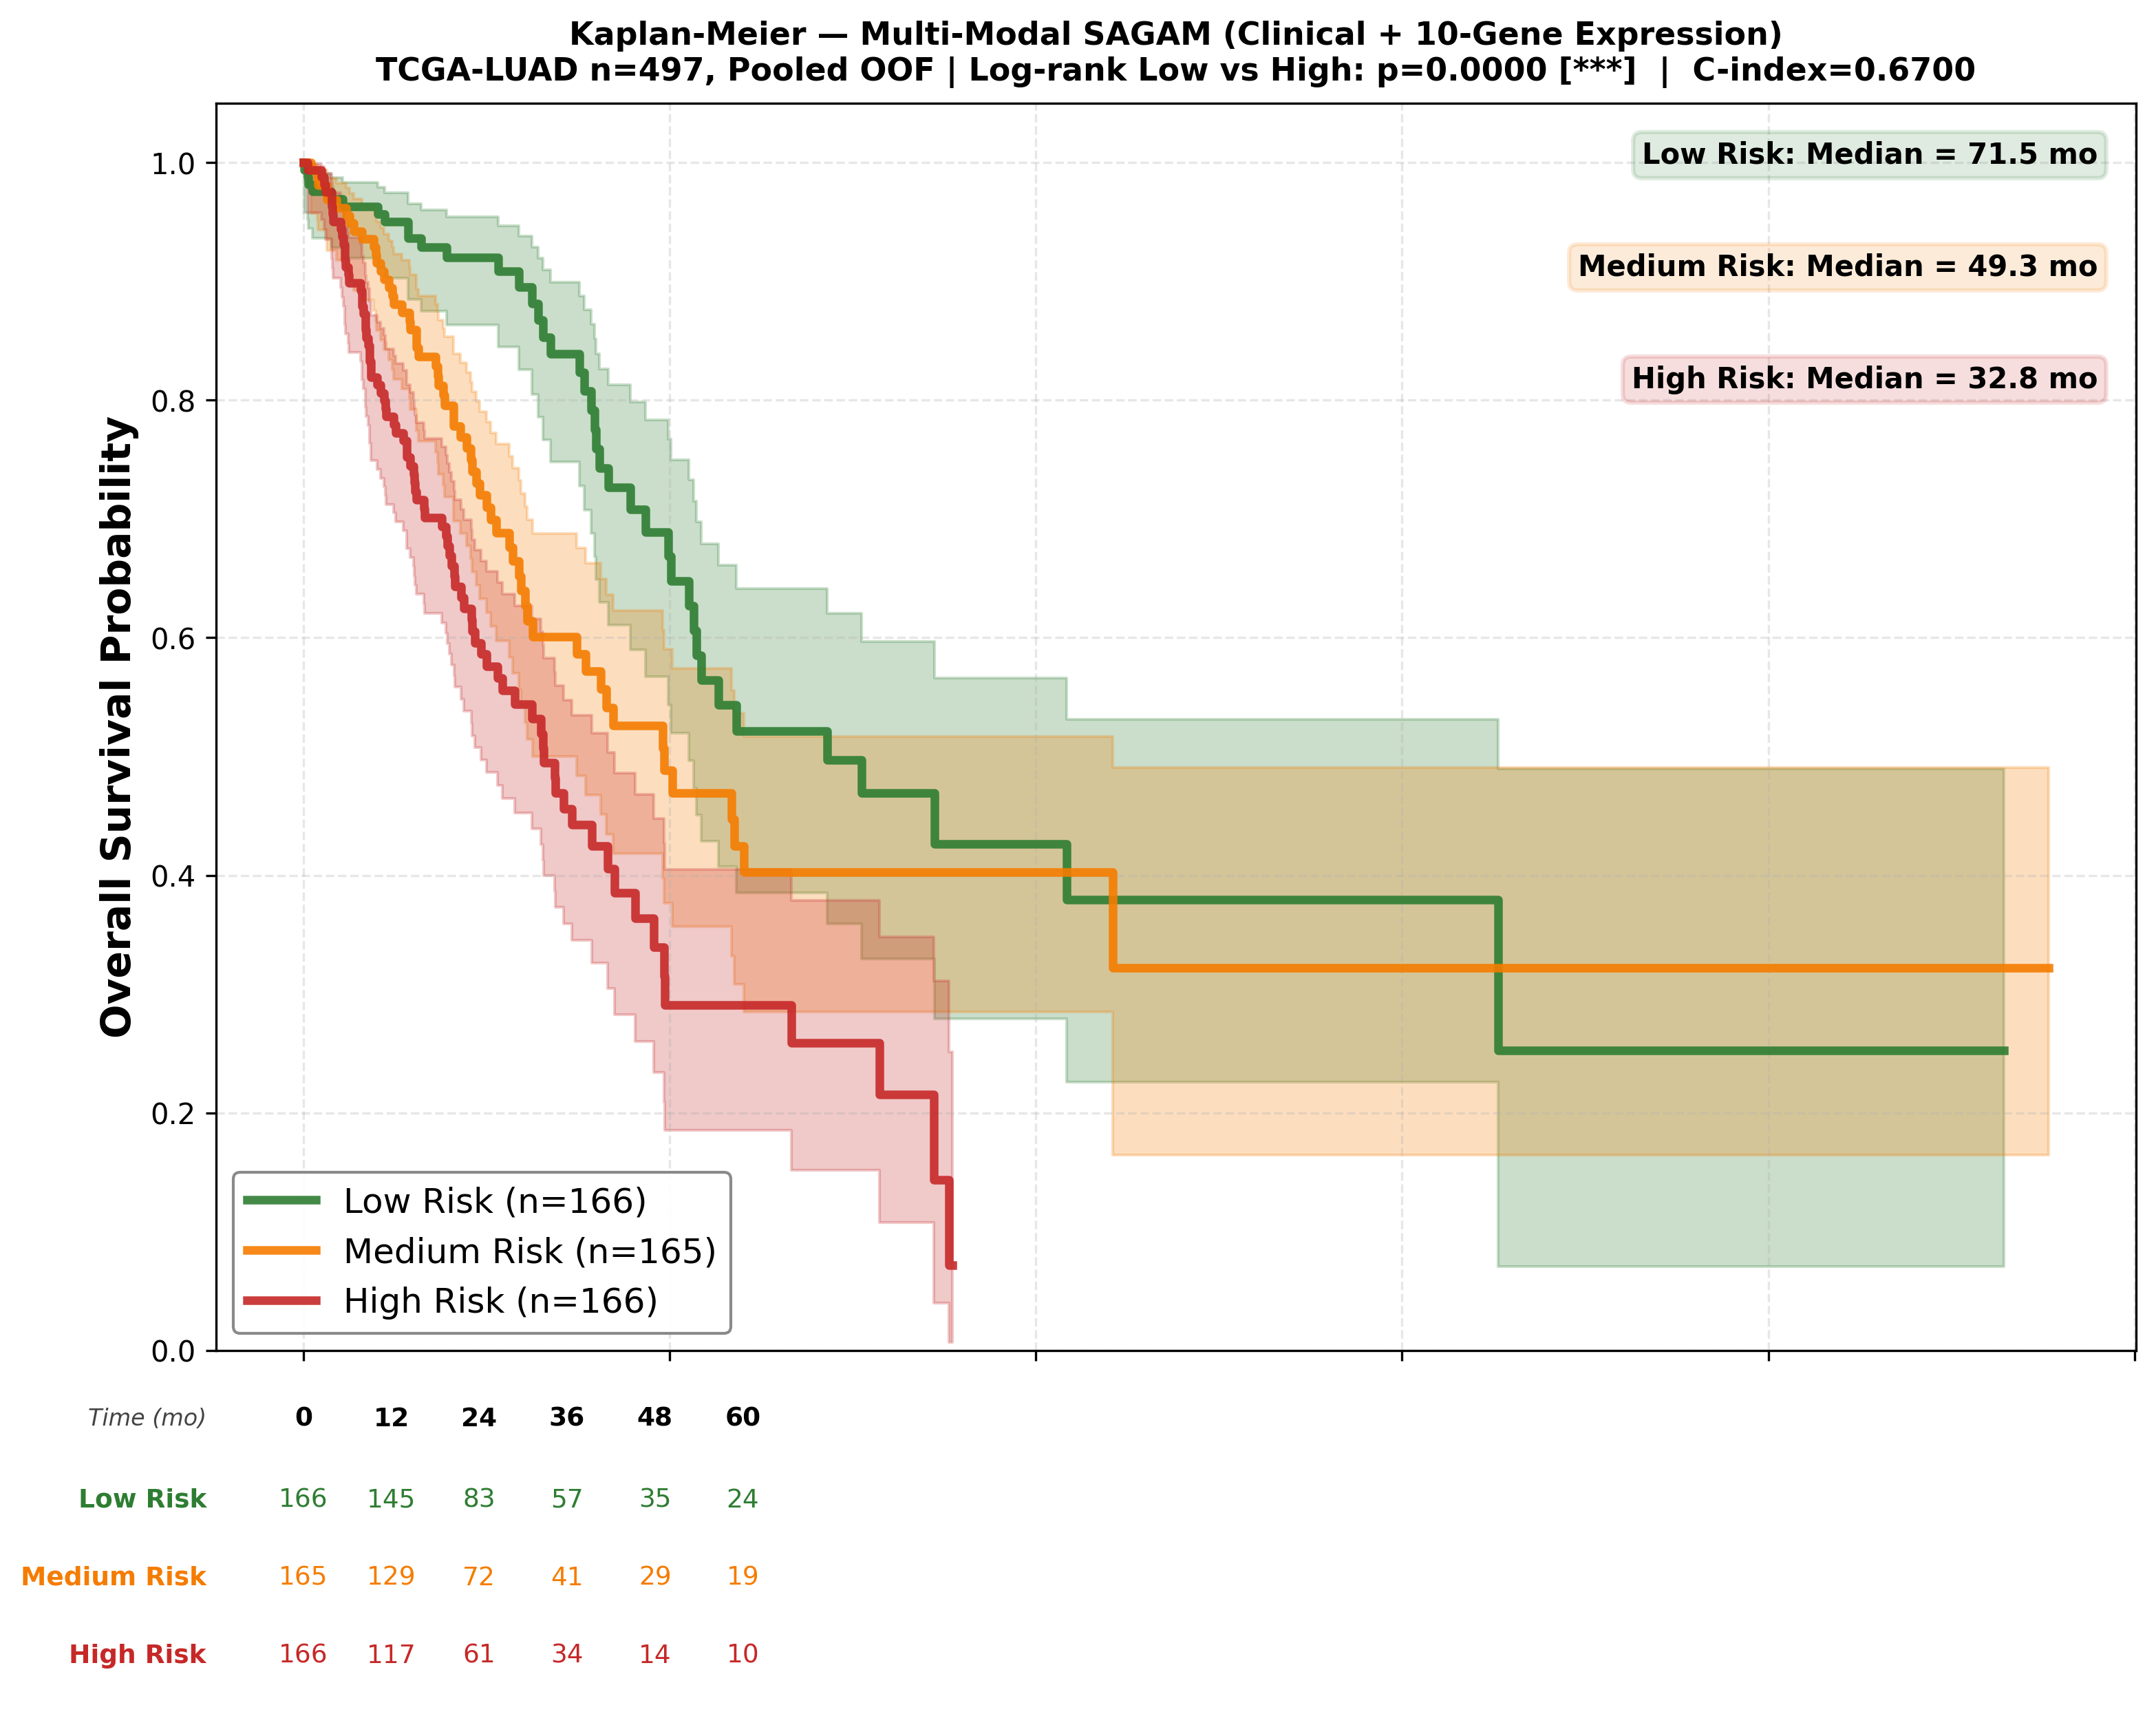
\includegraphics[width=\columnwidth]{kaplan_meier_multimodal.png}
\caption{Kaplan--Meier curves for Multi-Modal SAGAM risk tertiles on TCGA-LUAD
(pooled OOF scores). Log-rank (Low vs.\ High) $p<0.001$. The number-at-risk
table is shown beneath the curves.}
\label{fig:km}
\end{figure}

\begin{table}[!t]
\centering
\caption{Risk-tertile survival (Multi-Modal SAGAM, pooled OOF).}
\label{tab:km}
\begin{tabular}{lcccc}
\toprule
\textbf{Group} & \textbf{$n$} & \textbf{Median OS} & \textbf{HR (vs High)} & \textbf{$p$}\\
\midrule
Low    & $\approx$166 & 71.5 mo & 0.375 (0.257--0.547) & $<0.001$ \\
Medium & $\approx$166 & 49.3 mo & 0.728 (0.521--1.017) & $0.063$ \\
High   & $\approx$165 & 32.8 mo & Ref. & --- \\
\bottomrule
\end{tabular}
\end{table}

\subsection{Interpretability: Smooth Trust Functions}
Fig.~\ref{fig:smooths} shows the five learned contribution functions
$f_k(s_k)$ with their trust zones (shaded) and a dashed linear-equivalent
baseline. Summing absolute spline-coefficient magnitude per learner, GBS
dominates ($\approx$63\%), followed by DeepSurv ($\approx$30\%) and RSF
($\approx$7\%), with XGBoost-Cox and ExprCox each below 1\%. The GBS smooth is
a characteristic S-curve --- near-flat at low risk, a steep informative
transition in the mid-range, and a high-risk plateau --- exactly the nonlinear
weighting a single scalar cannot represent. The concentration of weight on GBS
and DeepSurv, with XGBoost and ExprCox near zero, also shows the meta-learner
performing implicit learner selection: redundant signal (expression captured by
the tree/network learners) is down-weighted automatically rather than
double-counted.

\begin{figure*}[!t]
\centering
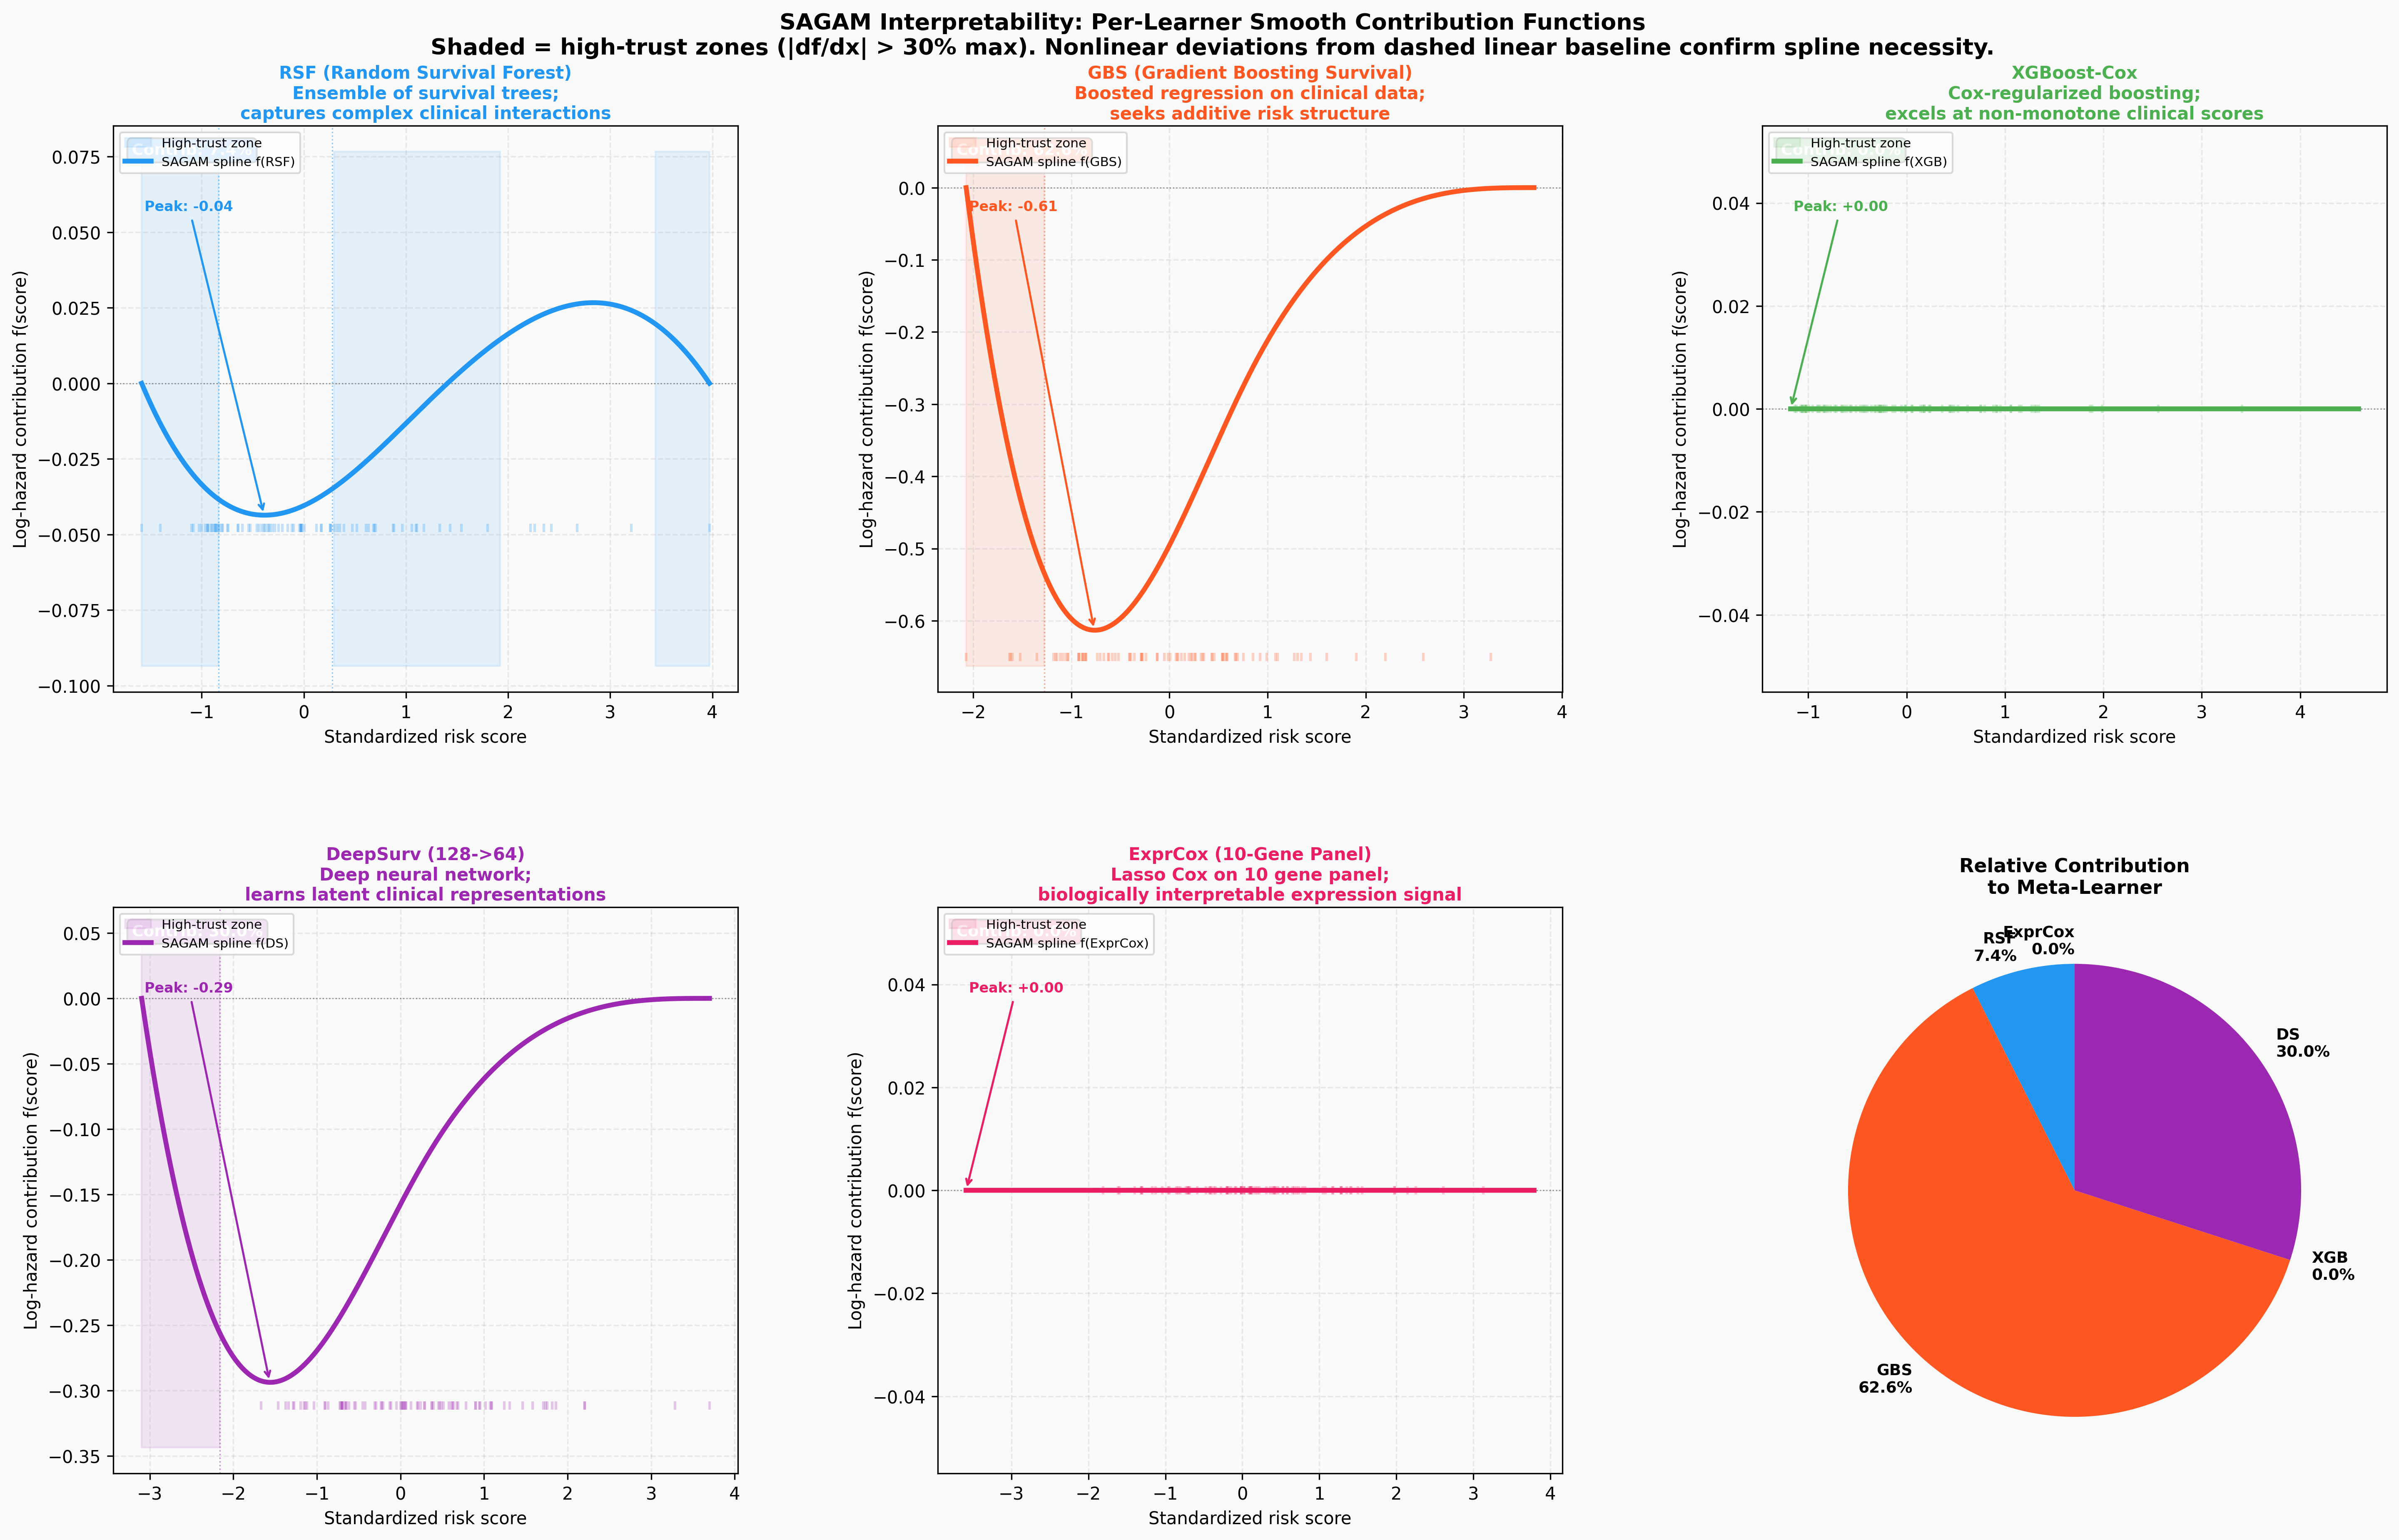
\includegraphics[width=0.95\textwidth]{interpretability_trust_zones.png}
\caption{Per-learner B-spline contribution functions $f_k(s_k)$ for
Multi-Modal SAGAM. Shaded bands are trust zones ($|f_k'|>30\%$ of its
maximum); dashed grey lines are the linear-equivalent fit. Deviations from the
dashed line quantify the nonlinearity the spline captures. The pie summarises
relative contribution: GBS $\approx$63\%, DeepSurv $\approx$30\%, RSF
$\approx$7\%, XGBoost-Cox and ExprCox $<$1\%.}
\label{fig:smooths}
\end{figure*}

\subsection{External Validation}
Table~\ref{tab:external} reports external results using the expression panel.
On GSE31210, SAGAM reaches $C{=}0.661$ (bootstrap 95\% CI 0.567--0.759),
the best of all tested models on that cohort (DeepSurv 0.626; RSF 0.541;
linear stacking 0.492), with log-rank $p=8.5{\times}10^{-4}$ --- highly
significant stratification on entirely independent data. On GSE68465, SAGAM
attains only $C{=}0.551$ ($p{=}0.093$, NS). We attribute the drop to three
measurable causes: (i) \emph{gene dropout} --- 3 of 10 panel genes are absent
from the HG-U133 Plus 2.0 probe set; (ii) \emph{event-rate mismatch} ---
52.3\% vs.\ 36.2\% in training, reflecting a different patient population; and
(iii) \emph{platform batch effects} between HG-U133A and Plus 2.0. This matches
the well-documented portability problem in expression-based
prognosis~\cite{luo2010comparison}, and we report it rather than omit it.

\begin{table}[!t]
\centering
\caption{External validation (10-gene expression panel).}
\label{tab:external}
\begin{tabular}{lccccc}
\toprule
\textbf{Cohort} & \textbf{$n$} & \textbf{Events} & \textbf{C-SAGAM} & \textbf{Log-rank $p$} & \textbf{Verdict}\\
\midrule
GSE31210 & 226 & 35  & \textbf{0.661} & $8.5{\times}10^{-4\,***}$ & pass \\
GSE68465 & 432 & 226 & 0.551 & $0.093$ (NS) & fail \\
\bottomrule
\end{tabular}
\end{table}

\subsection{Statistical Significance and Ablation}
Paired Wilcoxon signed-rank tests on the five fold-level C-indices place
SAGAM vs.\ Linear at $\Delta{=}{+}0.006$ ($p{=}0.31$), vs.\ DeepSurv at
$\Delta{=}{-}0.002$ ($p{=}0.63$), and vs.\ RSF at $\Delta{=}{+}0.014$
($p{=}0.09$). With only five paired observations these tests are
underpowered, and we present them transparently rather than over-claiming
significance. A spline degrees-of-freedom ablation (conducted on the
clinical-only configuration, where absolute C-indices are lower) confirms the
$J{=}4$ choice: C-index of 0.557 ($J{=}3$), \textbf{0.578} ($J{=}4$), 0.549
($J{=}5$), and 0.498 ($J{=}6$) --- $J{=}4$ is optimal, with higher $J$
overfitting the OOF scores.

% ── VI. DISCUSSION ───────────────────────────────────────────────────────────
\section{Discussion}
\label{sec:discussion}

\subsection{Why Multi-Modal Fusion Helps}
The $+0.050$ C-index gain and simultaneous halving of fold variance indicate
the expression panel supplies prognostic information orthogonal to staging,
plausibly reflecting immune (CD1B), invasion (RHOV, LYPD3), and Wnt/EGFR
(DKK1, FAM83A) biology. The variance reduction is as important as the mean
gain: a model that is reliable across folds is more trustworthy for deployment
than one that is occasionally excellent and occasionally poor.

\subsection{Interpretability as the Core Contribution}
The functions $f_k(s_k)$ in Eq.~\eqref{eq:smooth} are a genuine advance in
ensemble interpretability for survival. Unlike SHAP, which explains one
prediction at a time and post-hoc, the spline smooth is a global, continuous
object that is \emph{part of the model}. A clinician can read off, for a given
risk score, which components the ensemble is leaning on and whether it is
confident (steep) or deferring (flat). The automatic suppression of XGBoost
and ExprCox to near-zero weight is itself informative --- it reports redundancy
in the base suite.

\subsection{Limitations}
\textbf{External scope.} The GSE68465 result shows platform portability is
unresolved; probe-set imputation or quantile-normalisation
transfer~\cite{luo2010comparison} is needed before cross-platform deployment.
\textbf{Power.} Five outer folds limit the significance of paired comparisons;
repeated nested CV would help. \textbf{Short-horizon calibration.} The 1-year
tdAUC lags rank-optimised baselines; an IPCW-weighted Brier objective for the
meta-learner could close this. \textbf{Biological validation.} Risk groups are
not yet cross-referenced against EGFR/KRAS/ALK status, which would confirm that
SAGAM separates biologically distinct subtypes.

\subsection{Future Work}
Priorities: (1) panel recalibration for HG-U133 Plus 2.0; (2) EGFR/KRAS/ALK
mutation stratification; (3) comparison against published transformer/deep
survival baselines (SurvTRACE~\cite{wang2022survtrace},
DeepHit~\cite{lee2018deephit}); (4) extension to LUSC and other tumour types;
and (5) larger training cohorts (e.g., NLST).

% ── VII. CONCLUSION ──────────────────────────────────────────────────────────
\section{Conclusion}
\label{sec:conclusion}
We presented SAGAM, a multi-modal interpretable survival meta-learner whose
B-spline GAM combiner exposes, rather than hides, how an ensemble forms its
risk estimate. On TCGA-LUAD it attains $C{=}0.670\pm0.023$ under strict nested
cross-validation --- $+0.050$ over clinical-only and with half the fold
variance --- and stratifies patients into tertiles separated by 38.7 months of
median survival. External validation confirms generalisability to a matched
Affymetrix HG-U133A cohort ($C{=}0.661$, $p{=}0.0008$) and, just as
informatively, characterises where it fails. The central contribution is the
B-spline trust-function framework: a principled, visualisable account of
nonlinear, score-dependent learner reliance that linear stacking cannot
provide. Code, figures, and trained artefacts are released for full
reproducibility.

% ── References ───────────────────────────────────────────────────────────────
\begin{thebibliography}{99}

\bibitem{siegel2024cancer}
R.~L. Siegel, A.~N. Giaquinto, and A.~Jemal,
``Cancer statistics, 2024,''
\textit{CA Cancer J. Clin.}, vol.~74, no.~1, pp.~12--49, 2024.

\bibitem{cox1972regression}
D.~R. Cox, ``Regression models and life-tables,''
\textit{J. R. Stat. Soc. B}, vol.~34, no.~2, pp.~187--202, 1972.

\bibitem{simon2011regularization}
N.~Simon, J.~Friedman, T.~Hastie, and R.~Tibshirani,
``Regularization paths for Cox's proportional hazards model via coordinate descent,''
\textit{J. Stat. Softw.}, vol.~39, no.~5, pp.~1--13, 2011.

\bibitem{ishwaran2008random}
H.~Ishwaran, U.~B. Kogalur, E.~H. Blackstone, and M.~S. Lauer,
``Random survival forests,''
\textit{Ann. Appl. Stat.}, vol.~2, no.~3, pp.~841--860, 2008.

\bibitem{hothorn2006survival}
T.~Hothorn, P.~B\"uhlmann, S.~Dudoit, A.~Molinaro, and M.~J. van der Laan,
``Survival ensembles,''
\textit{Biostatistics}, vol.~7, no.~3, pp.~355--373, 2006.

\bibitem{chen2016xgboost}
T.~Chen and C.~Guestrin,
``XGBoost: A scalable tree boosting system,''
in \textit{Proc. ACM SIGKDD}, 2016, pp.~785--794.

\bibitem{katzman2018deepsurv}
J.~L. Katzman, U.~Shaham, A.~Cloninger, J.~Bates, T.~Jiang, and Y.~Kluger,
``DeepSurv: Personalised treatment recommender system using a Cox proportional hazards deep neural network,''
\textit{BMC Med. Res. Methodol.}, vol.~18, no.~24, 2018.

\bibitem{van2007super}
M.~J. van der Laan, E.~C. Polley, and A.~E. Hubbard,
``Super learner,''
\textit{Stat. Appl. Genet. Mol. Biol.}, vol.~6, no.~1, 2007.

\bibitem{polley2010super}
E.~C. Polley and M.~J. van der Laan,
``Super learner in prediction,''
\textit{U.C. Berkeley Div. Biostat. Working Papers}, 2010.

\bibitem{shedden2008gene}
K.~Shedden \textit{et~al.},
``Gene expression-based survival prediction in lung adenocarcinoma: a multi-site, blinded validation study,''
\textit{Nat. Med.}, vol.~14, no.~8, pp.~822--827, 2008.

\bibitem{beer2002gene}
D.~G. Beer \textit{et~al.},
``Gene-expression profiles predict survival of patients with lung adenocarcinoma,''
\textit{Nat. Med.}, vol.~8, no.~8, pp.~816--824, 2002.

\bibitem{luo2010comparison}
J.~Luo \textit{et~al.},
``A comparison of batch effect removal methods for enhancement of prediction performance using MAQC-II microarray gene expression data,''
\textit{Pharmacogenomics J.}, vol.~10, no.~4, pp.~278--291, 2010.

\bibitem{harrell1982evaluating}
F.~E. Harrell, R.~M. Califf, D.~B. Pryor, K.~L. Lee, and R.~A. Rosati,
``Evaluating the yield of medical tests,''
\textit{JAMA}, vol.~247, no.~18, pp.~2543--2546, 1982.

\bibitem{graf1999assessment}
E.~Graf, C.~Schmoor, W.~Sauerbrei, and M.~Schumacher,
``Assessment and comparison of prognostic classification schemes for survival data,''
\textit{Stat. Med.}, vol.~18, no.~17-18, pp.~2529--2545, 1999.

\bibitem{uno2007evaluating}
H.~Uno, T.~Cai, L.~Tian, and L.~J. Wei,
``Evaluating prediction rules for $t$-year survivors with censored regression models,''
\textit{J. Am. Stat. Assoc.}, vol.~102, no.~478, pp.~527--537, 2007.

\bibitem{lundberg2017unified}
S.~M. Lundberg and S.-I. Lee,
``A unified approach to interpreting model predictions,''
in \textit{Adv. Neural Inf. Process. Syst.}, vol.~30, 2017.

\bibitem{friedman2001greedy}
J.~H. Friedman,
``Greedy function approximation: A gradient boosting machine,''
\textit{Ann. Stat.}, vol.~29, no.~5, pp.~1189--1232, 2001.

\bibitem{aalen1989linear}
O.~O. Aalen,
``A linear regression model for the analysis of life times,''
\textit{Stat. Med.}, vol.~8, no.~8, pp.~907--925, 1989.

\bibitem{wang2022survtrace}
Z.~Wang, J.~Sun, and Z.~Jiang,
``SurvTRACE: Transformers for survival analysis with competing events,''
in \textit{Proc. ACM BCB}, 2022.

\bibitem{lee2018deephit}
C.~Lee, W.~R. Zame, J.~Yoon, and M.~van~der Schaar,
``DeepHit: A deep learning approach to survival analysis with competing risks,''
in \textit{Proc. AAAI}, 2018.

\end{thebibliography}

\end{document}
